\usetikzlibrary{positioning,arrows,automata}
\tikzset{G node/.style={circle,fill=white,draw,minimum size=0.75cm,inner sep=0pt},}
\begin{frame}
	\frametitle{\problemtitle}
	Problem: given a weighted cycle, pick some edges and vertices such that each vertex is connected to a
	marked vertex via a path.
	\vspace{1em}

	\begin{figure}[!h]
		\centering
		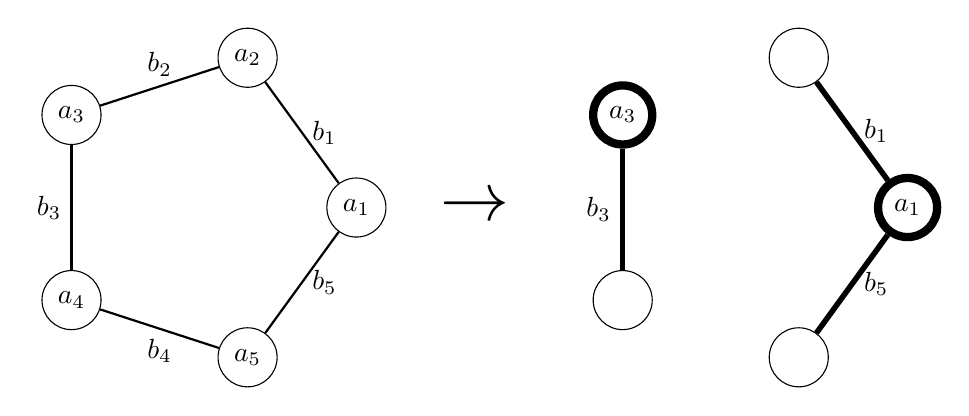
\begin{tikzpicture}
			\node[G node] (1) at ({2*cos(0 * 72)}, {2*sin(0 * 72)}) {$a_1$};
			\node[G node] (2) at ({2*cos(1 * 72)}, {2*sin(1 * 72)}) {$a_2$};
			\node[G node] (3) at ({2*cos(2 * 72)}, {2*sin(2 * 72)}) {$a_3$};
			\node[G node] (4) at ({2*cos(3 * 72)}, {2*sin(3 * 72)}) {$a_4$};
			\node[G node] (5) at ({2*cos(4 * 72)}, {2*sin(4 * 72)}) {$a_5$};
	
			\path[draw, thick]
				(1) edge node [right] {$b_1$} (2)
				(2) edge node [above] {$b_2$} (3)
				(3) edge node [left] {$b_3$} (4)
				(4) edge node [below] {$b_4$} (5)
				(5) edge node [right] {$b_5$} (1);

			\node[draw=white] at (3.5, 0) {\Huge $\rightarrow$};

			
			\node[G node, line width=3pt] (b1) at ({7+2*cos(0 * 72)}, {2*sin(0 * 72)}) {$a_1$};
			\node[G node] (b2) at ({7+2*cos(1 * 72)}, {2*sin(1 * 72)}) {$$};
			\node[G node, line width=3pt] (b3) at ({7+2*cos(2 * 72)}, {2*sin(2 * 72)}) {$a_3$};
			\node[G node] (b4) at ({7+2*cos(3 * 72)}, {2*sin(3 * 72)}) {$$};
			\node[G node] (b5) at ({7+2*cos(4 * 72)}, {2*sin(4 * 72)}) {$$};
	
			\path[draw, thick]
				(b1) [line width=2pt] edge node [right] {$b_1$} (b2)
				(b3) edge node [left] {$b_3$} (b4)
				(b5) edge node [right] {$b_5$} (b1);
		\end{tikzpicture}
	\end{figure}
\end{frame}

\begin{frame}
	\frametitle{\problemtitle}
	Idea: Add a central node for the concept of `power':
	\vspace{1em}

	\begin{figure}[!h]
		\centering
		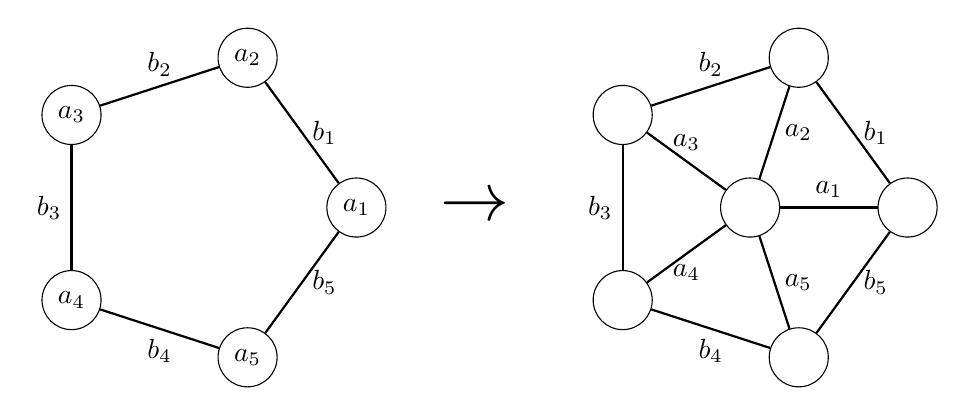
\begin{tikzpicture}
			\node[G node] (1) at ({2*cos(0 * 72)}, {2*sin(0 * 72)}) {$a_1$};
			\node[G node] (2) at ({2*cos(1 * 72)}, {2*sin(1 * 72)}) {$a_2$};
			\node[G node] (3) at ({2*cos(2 * 72)}, {2*sin(2 * 72)}) {$a_3$};
			\node[G node] (4) at ({2*cos(3 * 72)}, {2*sin(3 * 72)}) {$a_4$};
			\node[G node] (5) at ({2*cos(4 * 72)}, {2*sin(4 * 72)}) {$a_5$};
	
			\path[draw, thick]
				(1) edge node [right] {$b_1$} (2)
				(2) edge node [above] {$b_2$} (3)
				(3) edge node [left] {$b_3$} (4)
				(4) edge node [below] {$b_4$} (5)
				(5) edge node [right] {$b_5$} (1);

			\node[draw=white] at (3.5, 0) {\Huge $\rightarrow$};

			\node[G node] (1) at ({7+2*cos(0 * 72)}, {2*sin(0 * 72)}) {$$};
			\node[G node] (2) at ({7+2*cos(1 * 72)}, {2*sin(1 * 72)}) {$$};
			\node[G node] (3) at ({7+2*cos(2 * 72)}, {2*sin(2 * 72)}) {$$};
			\node[G node] (4) at ({7+2*cos(3 * 72)}, {2*sin(3 * 72)}) {$$};
			\node[G node] (5) at ({7+2*cos(4 * 72)}, {2*sin(4 * 72)}) {$$};
			\node[G node] (c) at (7, 0) {$$};
	
			\path[draw, thick]
				(1) edge node [right] {$b_1$} (2)
				(2) edge node [above] {$b_2$} (3)
				(3) edge node [left] {$b_3$} (4)
				(4) edge node [below] {$b_4$} (5)
				(5) edge node [right] {$b_5$} (1)
				(1) edge node [above] {$a_1$} (c)
				(2) edge node [right] {$a_2$} (c)
				(3) edge node [above] {$a_3$} (c)
				(4) edge node [below] {$a_4$} (c)
				(5) edge node [right] {$a_5$} (c);
		\end{tikzpicture}
	\end{figure}
\end{frame}

\begin{frame}
	\frametitle{\problemtitle}
	Now we just want to find the cheapest way to connect each vertex to the central node. But this is a
	classical minimum spanning tree problem $\rightarrow$ $O(n \log n)$.
	\vspace{1em}

	\begin{figure}[!h]
		\centering
		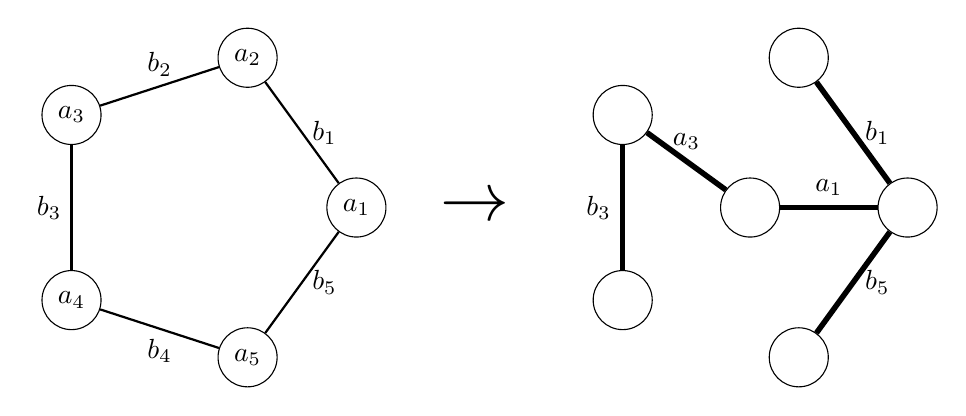
\begin{tikzpicture}
			\node[G node] (1) at ({2*cos(0 * 72)}, {2*sin(0 * 72)}) {$a_1$};
			\node[G node] (2) at ({2*cos(1 * 72)}, {2*sin(1 * 72)}) {$a_2$};
			\node[G node] (3) at ({2*cos(2 * 72)}, {2*sin(2 * 72)}) {$a_3$};
			\node[G node] (4) at ({2*cos(3 * 72)}, {2*sin(3 * 72)}) {$a_4$};
			\node[G node] (5) at ({2*cos(4 * 72)}, {2*sin(4 * 72)}) {$a_5$};
	
			\path[draw, thick]
				(1) edge node [right] {$b_1$} (2)
				(2) edge node [above] {$b_2$} (3)
				(3) edge node [left] {$b_3$} (4)
				(4) edge node [below] {$b_4$} (5)
				(5) edge node [right] {$b_5$} (1);

			\node[draw=white] at (3.5, 0) {\Huge $\rightarrow$};

			\node[G node] (1) at ({7+2*cos(0 * 72)}, {2*sin(0 * 72)}) {$$};
			\node[G node] (2) at ({7+2*cos(1 * 72)}, {2*sin(1 * 72)}) {$$};
			\node[G node] (3) at ({7+2*cos(2 * 72)}, {2*sin(2 * 72)}) {$$};
			\node[G node] (4) at ({7+2*cos(3 * 72)}, {2*sin(3 * 72)}) {$$};
			\node[G node] (5) at ({7+2*cos(4 * 72)}, {2*sin(4 * 72)}) {$$};
			\node[G node] (c) at (7, 0) {$$};
	
			\path[draw, thick]
				(1) [line width=2pt] edge node [right] {$b_1$} (2)
				(3) edge node [left] {$b_3$} (4)
				(5) edge node [right] {$b_5$} (1)
				(1) edge node [above] {$a_1$} (c)
				(3) edge node [above] {$a_3$} (c);
		\end{tikzpicture}
	\end{figure}
	Note: this works for any graph $G$, not just cycles!
\end{frame}
